\tikzset{every loop/.style={min distance=10mm,in=60,out=120,looseness=10}}

\begin{frame}{Two undecidable problems}

  \begin{block}{Theorem}
    The following problems are undecidable.
  \end{block}

  \begin{alertblock}{Determinisability problem}
    \begin{itemize}
	\item \textbf{Input} : a timed automaton $\mathcal{A}$.
	\item \textbf{Output} : yes if there exists a deterministic timed automaton $\mathcal{B}$ such that $\mathcal{L}(\mathcal{A}) = \mathcal{L}(\mathcal{B})$, else no.
    \end{itemize}
  \end{alertblock}
  
    \begin{alertblock}{Complementability problem}
    \begin{itemize}
	\item \textbf{Input} : a timed automaton $\mathcal{A}$.
	\item \textbf{Output} : yes if there exists a timed automaton $\mathcal{B}$ such that $\mathcal{L}(\mathcal{A})^c = \mathcal{L}(\mathcal{B})$, else no.
    \end{itemize}
  \end{alertblock}

\end{frame}


\begin{frame}{Proof: Lemma}

   \begin{block}{Notation}
    Let $A$ be the language of words of the form $t_1.a\dots t_n.a$ such that there exists a pair of $a$ separated by a time distance $1$:
$$\exists i,j [\![1,n]\!], i < j  \land  t_{i+1} + \dots + t_j = 1$$
  \end{block}

  \begin{block}{Property}
    The language $A$ is timed regular.\\
    The language $A^c$ is not timed regular.
  \end{block}

  \begin{block}{Proof idea}
    If there existed a timed automaton accepting $A^c$, it would need an unbounded number of clocks.\\
  \end{block}

\end{frame}



\begin{frame}{Proof: Lemma}

\begin{center}
\begin{figure}
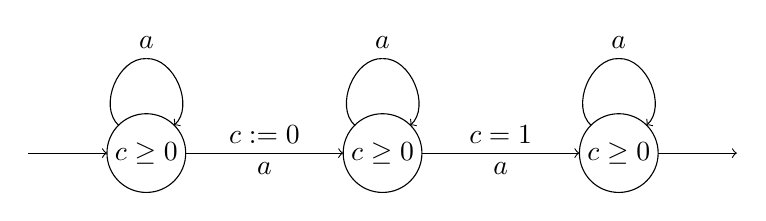
\begin{tikzpicture}
	\draw[->] (-1.5,0) -- (-0.5,0) ;

	\draw(0,0) circle (0.5) ;
	\draw (0,0) node{$c \geq 0$};
	%\path[->] (0,0.5) edge  [loop above] node {$a$} ();

	\draw (-0.35,0.35)        to [bend left=70] (0,1.2);
	\draw [->] (0,1.2)        to [bend left=70] (0.35,0.35);
	\draw (0,1.2) node[above]{$a$} ;

	\draw[->] (0.5,0) -- node[above]{$c := 0$} node[below]{$a$}(2.5,0) ;
	\draw(3,0) circle (0.5) ;
	\draw (3,0) node{$c \geq 0$};
	%\path[->] (3,0.5) edge  [loop above] node {$a$} ();

	\draw (2.65,0.35)        to [bend left=70] (3,1.2);
	\draw [->] (3,1.2)        to [bend left=70] (3.35,0.35);
	\draw (3,1.2) node[above]{$a$} ;

	\draw[->] (3.5,0) -- node[above]{$c = 1$} node[below]{$a$} (5.5,0) ;
	\draw(6,0) circle (0.5) ;
	\draw (6,0) node{$c \geq 0$};
	%\path[->] (6,0.5) edge  [loop above] node {$a$} ();

	\draw (5.65,0.35)        to [bend left=70] (6,1.2);
	\draw [->] (6,1.2)        to [bend left=70] (6.35,0.35);
	\draw (6,1.2) node[above]{$a$} ;

	\draw[->] (6.5,0) -- (7.5,0) ;

\end{tikzpicture}
\caption{Automaton accepting the language $A$}
\label{fig1}
\end{figure}
\end{center}

\end{frame}




\begin{frame}{Proof: the reduction}

	\begin{block}{Notation}
	    $\Sigma$ is an alphabet containing $a$ ; $c$ is a letter not in $\Sigma$. $\Gamma = \Sigma \cup \{c\}$.
  	\end{block}

	\begin{block}{Goal}
		Input of the universability problem: $L$, a timed regular language over $(\mathbb{R}\times\Sigma)^*$.\\
		Build the reduction from the universability problem to the determinisability and complementability problem.\\
  	\end{block}

	\begin{block}{Notation}
		\begin{itemize}
			\item $\mathcal{L}_1 = L.(\mathbb{R} \times \{c\}).(\mathbb{R}\times\Sigma)^*$
			\item $\mathcal{L}_2$: set of words over $\Sigma$ with no $c$ or at least two $c$.
			\item $\mathcal{L}_3 = (\mathbb{R}\times\Sigma)^*.(\mathbb{R} \times \{c\}).A$
		\end{itemize}
  	\end{block}

\end{frame}


\begin{frame}{Proof: the reduction}

	\begin{block}{Notation}
		$\mathcal{L} = \mathcal{L}_1 \cup \mathcal{L}_2 \cup \mathcal{L}_3$ is the input to equivalence with a deterministic timed automaton and acceptation of the complement, built from $L$.
	\end{block}

	\begin{block}{Property}
		$\mathcal{L} = \mathcal{L}_1 \cup \mathcal{L}_2 \cup \mathcal{L}_3$ is timed regular, since $L$ and $A$ are timed regular.
	\end{block}

	\begin{block}{Lemma}
		If $L$ is universal, then $\mathcal{L}$ is accepted by a deterministic timed automaton, and $\mathcal{L}^c$ is accepted by a timed automaton.
	\end{block}

	\begin{block}{Proof}
		Easy: if $L = (\mathbb{R}\times\Sigma)^*$, then $\mathcal{L} = (\mathbb{R}\times\Gamma)^*$ and $\mathcal{L}^c = \emptyset$.
	\end{block}

	
\end{frame}


\begin{frame}{Proof: the reduction}

	\begin{block}{Lemma}
		If $L \subsetneq (\mathbb{R}\times\Sigma)^*$, then $\mathcal{L}^c$ is not timed regular.
	\end{block}
	
	\begin{block}{Proof}
	Let $u = t_1.a_1\dots t_n.a_n \not\in L$, and $x \in (\mathbb{R}\times\Sigma)^*$. Then $u.1.c.x \in \mathcal{L}$ iff $x \in A$. Thus, $u.1.c.x \in \mathcal{L}^c$ iff $x \in A^c$.\\
	\textbf{Proof of not-regularity of $\mathcal{L}^c$: similar to the one of $x \in A^c$, which is not detailed.}
	\end{block}

\end{frame}


\begin{frame}{Clock Minimization Problem}

  \begin{alertblock}{Minimization of the number of clocks}
    Given $\mathcal{A}$ a timed automaton with $n$ clocks, is there an automaton $\mathcal{B}$ with $n-1$ clocks such that $\mathcal{L(B)=L(A)}$? If so, construct $\mathcal{B}$.\\
    This problem is known to be \textbf{undecidable}.
  \end{alertblock}
  \vfill
  \begin{exampleblock}{What if we don't ask for a witness?}
    Simply answer Yes or No if the number of clocks can be reduced (decision problem).
  \end{exampleblock}
    
\end{frame}

\begin{frame}{Back to clock minimization}
  
  \begin{alertblock}{Undecidable problem}
    Given $\mathcal{A}$ a timed automaton with $n$ clocks, is there an automaton $\mathcal{B}$ with $n-1$ clocks such that $\mathcal{L(B)=L(A)}$?
  \end{alertblock}

  Give idea of the proof.
  
\end{frame}
